% Copyright (c) 2017 Benito Palacios Sánchez - All Rights Reserved.
% Esta obra está licenciada bajo la Licencia Creative Commons Atribución 4.0
% Internacional. Para ver una copia de esta licencia, visita
% http://creativecommons.org/licenses/by/4.0/.

% Template
\documentclass[usenames,dvipsnames]{beamer}
\pdfoutput=1

% Notes. Uncomment to view the notes.
%\setbeameroption{show notes}
%\setbeamertemplate{note page}[plain]    % Remove the note page style

% Load this package to allow load many big packages.
\usepackage{etex}

% Font
\usepackage[T1]{fontenc}        % Output font
\usepackage[utf8]{inputenc}     % Input encoding
\usepackage[spanish]{babel}     % For Spanish texts
\usepackage{FiraSans}           % For FiraSans beauty fonts

% Theme
\usetheme{Darmstadt}
\usecolortheme{whale}

% Other packages
\usepackage{xcolor}             % For color in text
\usepackage{url}                % For links
\usepackage{pifont}             % For tick symbol
\usepackage{graphicx}           % For graphics
\usepackage{epstopdf}           % For EPS graphics in Windows
\usepackage{multimedia}         % For media
\usepackage{verbatim}           % For non-parsed text blocks
\usepackage{tikz}               % To draw over images
\usepackage{ctable}             % For tables
\usepackage{textcomp}           % For text arrows.
\usepackage{listings}           % For blocks of code
\lstset{language=[Sharp]C,basicstyle=\scriptsize\ttfamily, keywordstyle=\scriptsize\color{blue}\ttfamily}

% My package
\usepackage{../Layout}

% Information about author and document
\title{Introducción al ROM Hacking}
\subtitle{Primeros pasos}
\date[Marzo de 2017]{24 de marzo de 2017}
\author{Benito Palacios}
\authortitle{}
\authoremail{benito.palaciossanchez.es@ieee.org}
\institute[IEEE SB UGR]{Rama estudiantil de IEEE en la UGR}
\titlelogo{../logo.png}

% Add a little logo in the corner of the slides
\pgfdeclareimage[height=0.5cm]{logo-mini}{../logo_mini.png}
\logo{\pgfuseimage{logo-mini}}

\begin{document}

    % Title page
    {
    \usebackgroundtemplate{
        \includegraphics[width=\paperwidth]{../background.jpg}}
    \begin{frame}[plain]
        \titlepage{}
    \end{frame}
    }

    % Content
    \section{Introducción}
\subsection{Sobre mi\ldots}
\begin{frame}{¿Quién soy?}
    \begin{columns}
    \begin{column}{0.75\textwidth}
        \Large
        Benito Palacios \\
        \textbf{@pleonex}
    \end{column}
    \begin{column}{0.25\textwidth}
        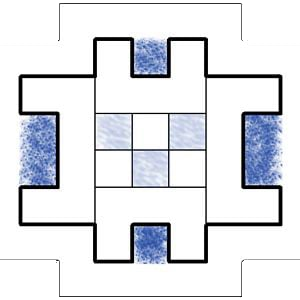
\includegraphics[width=\textwidth]{imgs/pleonex.png}
    \end{column}
    \end{columns}

    \vfill{}
    \setlength{\leftmargini}{0em}
    \begin{itemize}
        \item<2-> Graduado en Ingeniería de Tecnologías de Telecomunicación
        \begin{itemize}
            \item <2-> Trabajo Fin de Grado sobre seguridad en videojuegos
        \end{itemize}
        \item<3-> Miembro fundador de IEEE Student Branch of Granada
        \item<4-> \textgreater 7 años en el mundo del ROM Hacking
        \item<5-> Miembro de GradienWords
    \end{itemize}
    \visible<5->{
        \leavevmode\makebox(0,0){
        \put(250, 75){\includegraphics[width=0.15\textwidth]{imgs/gradienwords.png}}}}
\end{frame}

\subsection{Mis proyectos}
\begin{frame}{Tinke}
    \centering
    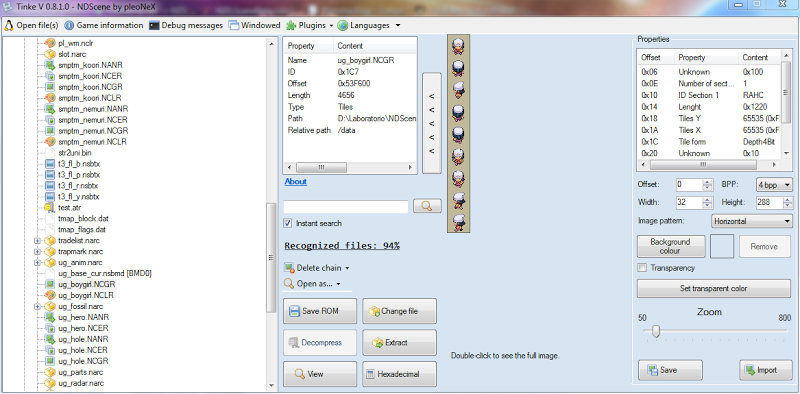
\includegraphics[width=0.65\textwidth]{imgs/tinke_preview.png}
    \vfill
    \includegraphics[width=0.22\textwidth]{imgs/tinke1.png}
    \hfill
    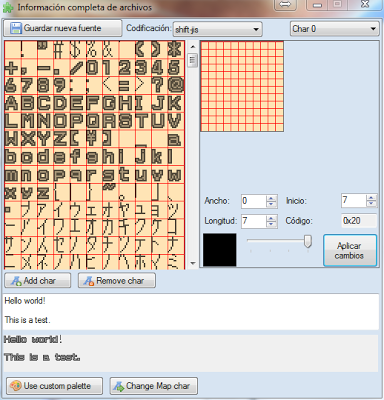
\includegraphics[width=0.22\textwidth]{imgs/tinke2.png}
    \hfill
    \includegraphics[width=0.22\textwidth]{imgs/tinke3.png}
    \hfill
    \includegraphics[width=0.22\textwidth]{imgs/tinke4.png}
\end{frame}

\begin{frame}{Ninokuni: El Mago de las Tinieblas}
    \centering
    \includegraphics[width=0.4\textwidth]{imgs/ninokuni_preview.jpg}
    \vfill
    \includegraphics[width=0.2\textwidth]{imgs/nino1.png}
    \hfill
    \includegraphics[width=0.2\textwidth]{imgs/nino2.png}
    \hfill
    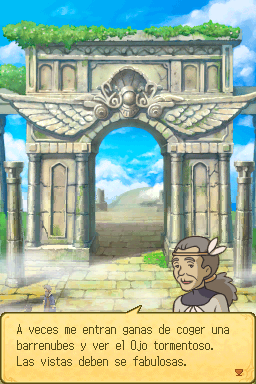
\includegraphics[width=0.2\textwidth]{imgs/nino3.png}
    \hfill
    \includegraphics[width=0.2\textwidth]{imgs/nino4.png}
\end{frame}

\begin{frame}{Fan traducciones}
    \setlength{\leftmargini}{0em}
    \begin{columns}
    \begin{column}{0.5\textwidth}
        \begin{itemize}
            \item<1-> Pokémon Conquest
            \item<2-> Final Fantasy: Four Heroes
        \end{itemize}
        \vfill
        \visible<3->{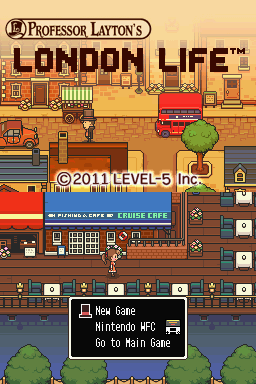
\includegraphics[width=0.4\textwidth]{imgs/london_life.png}}
        \hfill
        \visible<4->{\includegraphics[width=0.4\textwidth]{imgs/sff.png}}
    \end{column}
    \begin{column}{0.5\textwidth}
        \visible<1->{\includegraphics[width=0.4\textwidth]{imgs/pokconquest.png}}
        \hfill
        \visible<2->{\includegraphics[width=0.4\textwidth]{imgs/ff4ol.png}}
        \vfill
        \begin{itemize}
            \item<3-> Profesor Layton: London Life
            \item<4-> Shining Force Feather
        \end{itemize}
    \end{column}
    \end{columns}
\end{frame}

\subsection{¿Qué es ROM Hacking?}
\begin{frame}{Érase una vez\ldots}
    \centering \includegraphics[width=0.65\textwidth]{imgs/bigbang.jpg}
\end{frame}

\begin{frame}{¿Qué es un fichero?}
    \centering\fontsize{80}{0}\selectfont
    ¿ \includegraphics{imgs/file.png}~?
    \note{
      ¿Qué hay en el fichero para que luego podamos ver imágenes y
      escuchar música?
      ¿Cómo vemos esos bytes que luego se transforman en media?}
\end{frame}

\begin{frame}{La parte cruda de los archivos}
    \includefigure{BMP visto con editor hexadecimal HxD}{imgs/hexview.png}{0.6}
\end{frame}

\begin{frame}[fragile]{Especificaciones (BMP)}
    \footnotesize
    \ctable[]{ccl}{}{                                                       \FL
        Posición      & Tamaño        & Descripción                         \ML
        \multicolumn{3}{c}{Cabecera estándar}                               \NN
        \texttt{0x00} & \texttt{0x02} & \textit{Magic stamp}: \texttt{BM}   \NN
        \texttt{0x02} & \texttt{0x04} & Tamaño del fichero                  \NN
        \texttt{0x06} & \texttt{0x04} & Reservado                           \NN
        \texttt{0x0A} & \texttt{0x04} & Puntero a los datos de la imagen    \ML
        \multicolumn{3}{c}{Cabecera DIB}                                    \NN
        \texttt{0x00} & \texttt{0x04} & Tamaño de esta cabecera             \NN
        \texttt{0x04} & \texttt{0x04} & Ancho de la imagen                  \NN
        \texttt{0x06} & \texttt{0x04} & Alto de la imagen                   \NN
        \texttt{0x08} & \texttt{0x02} & Número de planos de color (1)       \NN
        \texttt{0x0A} & \texttt{0x02} & Número de bits por píxel            \ML
        \multicolumn{3}{c}{Paleta de colores}                               \ML
        \multicolumn{3}{c}{Píxeles}                                         \LL
    }
\end{frame}

\begin{frame}{Especificaciones (BMP)}
    \begin{columns}
    \begin{column}[T]{0.7\textwidth}
        \begin{tikzpicture}
        \node[anchor=south west,inner sep=0] (image) at (0,0)
        {\includegraphics[width=\textwidth]{imgs/hexview.png}};
            \begin{scope}[x={(image.south east)},y={(image.north west)}]
                \draw<1,6->[red,semithick] (0.15,0.785) rectangle (0.64,0.76);
                \draw<2-5>[red,semithick] (0.15,0.76) rectangle (0.22,0.785);
                \draw<3-5>[red,semithick] (0.22,0.76) rectangle (0.36,0.785);
                \draw<4-5>[red,semithick] (0.36,0.76) rectangle (0.50,0.785);
                \draw<5>[red,semithick] (0.50,0.76) rectangle (0.64,0.785);
                \draw<6,13->[green,semithick] (0.64,0.76) -- (0.64,0.785) -- (0.72,0.785) -- (0.72,0.605) -- (0.50,0.605) -- (0.50,0.58) -- (0.15,0.58) -- (0.15,0.76) -- (0.64,0.76);
                \draw<7-12>[green,semithick] (0.72,0.76) -- (0.64,0.76) -- (0.64,0.785) -- (0.72,0.785);
                \draw<7-12>[green,semithick] (0.15,0.76) -- (0.22,0.76) -- (0.22,0.735) -- (0.15,0.735);
                \draw<8-12>[green,semithick] (0.22,0.735) rectangle (0.36,0.76);
                \draw<9-12>[green,semithick] (0.36,0.735) rectangle (0.50,0.76);
                \draw<10-12>[green,semithick] (0.50,0.735) rectangle (0.57,0.76);
                \draw<11-12>[green,semithick] (0.57,0.735) rectangle (0.64,0.76);
                \draw<12>[green,semithick] (0.64,0.735) -- (0.64,0.76) -- (0.72,0.76) -- (0.72,0.605) -- (0.50,0.605) -- (0.50,0.58) -- (0.15,0.58) -- (0.15,0.735) -- (0.64,0.735);
                \draw<13->[blue,semithick] (0.15,0.12) -- (0.15,0.58) -- (0.50,0.58) -- (0.50,0.605) -- (0.72,0.605) -- (0.72, 0.145) -- (0.50,0.145) -- (0.50,0.12) -- (0.15,0.12);
                \draw<14->[black,semithick] (0.15,0.04) -- (0.15,0.12) -- (0.50,0.12) -- (0.50,0.145) -- (0.72,0.145) -- (0.72,0.04) ;
            \end{scope}
        \end{tikzpicture}
    \end{column}
    \hfill
    \begin{column}[T]{0.4\textwidth}
        \begin{enumerate}
            \item<1-> Cabecera estándar
            \begin{enumerate}
                \item<2-> \textit{Magic stamp}
                \item<3-> Tamaño fichero
                \item<4-> Reservado
                \item<5-> Puntero datos
            \end{enumerate}
            \item<6-> Cabecera DIB
            \begin{enumerate}
                \item<7-> Tamaño DIB
                \item<8-> Ancho
                \item<9-> Alto
                \item<10-> Planos de color
                \item<11-> BPP
                \item<12-> Meta-datos
            \end{enumerate}
            \item<13-> Paleta
            \item<14-> Píxeles
        \end{enumerate}
    \end{column}
    \end{columns}
\end{frame}

\begin{frame}{¿Qué hay dentro de un juego?}
    \fontsize{45}{0}\selectfont
    \begin{columns}
    \begin{column}{0.70\textwidth}
        ¿ \includegraphics{imgs/gamefile.png}~?
        \visible<2->{\textrightarrow}
    \end{column}
    \begin{column}{0.30\textwidth}
        \visible<2->{\includegraphics[width=\textwidth]{imgs/game_desmume.png}}
    \end{column}
    \end{columns}
\end{frame}

\begin{frame}{La parte cruda de un juego}
    \includegraphics[width=\textwidth]{imgs/game_hex.png}
\end{frame}

\begin{frame}{¿Y ahora? ¿Y la especificación?}
    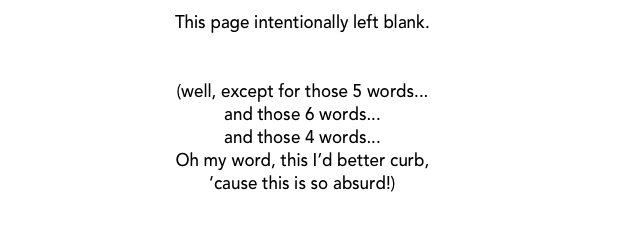
\includegraphics[width=\textwidth]{imgs/left_blank.png}
\end{frame}

\begin{frame}{ROM Hacking}
    \includegraphics[width=\textwidth]{imgs/this_is_romhacking.png}
\end{frame}

\begin{frame}{ROM Hacking}
    \begin{columns}
    \begin{column}{0.35\textwidth}
        Propósito:
        \begin{itemize}
            \item<2-> Fan traducciones
            \item<3-> Mods
            \item<4-> Extraer recursos
            \item<5-> Curiosidad
        \end{itemize}
    \end{column}
    \begin{column}{0.65\textwidth}
        \centering
        \visible<2->{\includegraphics[width=0.45\textwidth]{imgs/ninokuni_preview.jpg}}
        \visible<3->{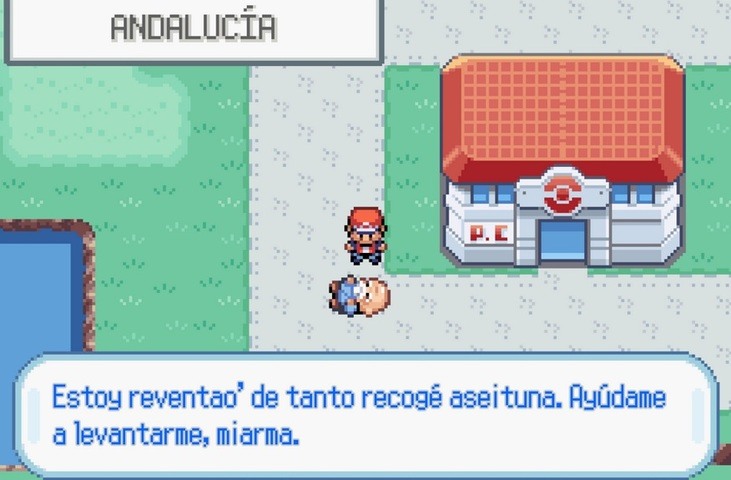
\includegraphics[width=0.45\textwidth]{imgs/mods_preview.jpg}}
        \visible<4->{\includegraphics[width=0.4\textwidth]{imgs/spriters.png}}
        \visible<5->{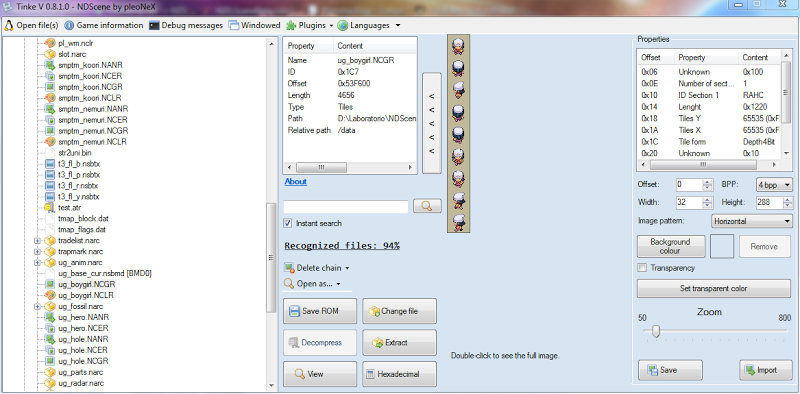
\includegraphics[width=0.8\textwidth]{imgs/tinke_preview.png}}
    \end{column}
    \end{columns}
\end{frame}

\subsection{Temario}
\begin{frame}[t]{Contenido del curso}
    \centering
    {\Large \textbf{IEEEsbUGR ROM Hacking Group}}
    \vfill
    \setlength{\leftmargini}{8em}
    \begin{enumerate}
        \addtolength{\itemsep}{10pt}
        \item Introducción al ROM Hacking
        \begin{enumerate}
            \item Introducción
            \item Hello World!
            \item Reto 1
            \item Textos
            \item Imágenes
            \item Media
            \item Reto 2
        \end{enumerate}
        \item Proyecto
        \item Presentación y taller
    \end{enumerate}
\end{frame}

    \section{Hello World!}
\begin{frame}{Hello World!}
    \Huge\centering\textbf{ROM HACKING TIME!}
\end{frame}

\subsection{NitroROM}
\begin{frame}{Especificación de juegos de NDS}
    \begin{block}{GBATEK}
        \centering
         Gameboy Advance / Nintendo DS / DSi - Technical Info \\
         Trabajo de Martin Korth en el desarrollo de no\$gba.
        \url{http://problemkaputt.de/gbatek.htm}
    \end{block}
    \vfill
    \small
    \begin{columns}
    \begin{column}{0.3\textwidth}
        \uncover<2->{Cabecera\\}
        \uncover<3->{Binario ARM9\\}
        \uncover<3->{Overlays ARM9}
    \end{column}
    \begin{column}{0.3\textwidth}
        \uncover<3->{Binario ARM7\\}
        \uncover<3->{Overlays ARM7\\}
        \uncover<4->{File Name Table}
    \end{column}
    \begin{column}{0.3\textwidth}
        \uncover<4->{File Allocation Table\\}
        \uncover<5->{Banner\\}
        \uncover<6->{Archivos}
    \end{column}
    \end{columns}
\end{frame}

\subsection{Conceptos}
\begin{frame}[fragile]{Números hexadecimales}
    \begin{uncoverenv}<2->Decimal: 0 1 2 3 4 5 6 7 8 9
    \begin{lstlisting}
    0 1 2 3 4 5 6 7 8 9 10 11 12 13 ...\end{lstlisting}\end{uncoverenv}

    \begin{uncoverenv}<3->Binario: 0 1
    \begin{lstlisting}
    0 1 10 11 100 101 110 111 1000 ...
    0 1  2  3   4   5   6   7    8\end{lstlisting}\end{uncoverenv}

    \begin{uncoverenv}<4->Octal: 0 1 2 3 4 5 6 7
    \begin{lstlisting}
    0 1 2 3 4 5 6 7 10 11 12 13 14 ...
    0 1 2 3 4 5 6 7  8  9 10 11 12\end{lstlisting}\end{uncoverenv}

    \begin{uncoverenv}<5->Hexadecimal: 0 1 2 3 4 5 6 7 8 9 A B C D E F
    \begin{lstlisting}
    0 1 2 3 4 5 6 7 8 9  A  B  C  D  E  F 10 11 12 ...
    0 1 2 3 4 5 6 7 8 9 10 11 12 13 14 15 16 17 18\end{lstlisting}\end{uncoverenv}
\end{frame}

\begin{frame}[fragile]{Números hexadecimales}
    \begin{wideitemize}
        \item<1-> Prefijo \texttt{0x} o sufijo \texttt{h} \\
        \texttt{0xA, FBh, 0xCA, FEh}

        \item<2-> Fácil representación de enteros:
    \end{wideitemize}
    \visible<2->{\footnotesize\ctable[]{cccccl}{}{                          \FL
        \# & Rango & Ejemplo & Bytes & Bits & Otros nombres                 \ML
        1 & \texttt{[0, 15]} & \texttt{0xC} & \textonehalf & 4 &            \NN
        2 & \texttt{[0, 255]} & \texttt{0xC0} & 1 & 8 & byte                \NN
        4 & \texttt{[0, 65,535]} & \texttt{0x0200} & 2 & 16 & ushort, WORD  \NN
        8 & \texttt{[0, 4,294,967,295]} & \texttt{0xB7000000} & 4 & 32 & uint, DWORD \LL
    }}
\end{frame}

\begin{frame}{Endianness}
    \begin{block}{}
        Orden en el que se guardan los bytes que forman valores mayores a 8 bits (ushort, uint, ulong, \ldots). MSB \textrightarrow LSB.
    \end{block}
    \centering{}\uncover<2->{Big Endian:}
    \visible<2->{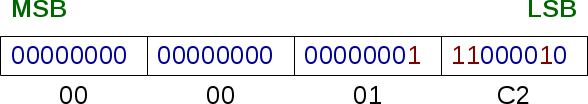
\includegraphics[width=0.9\textwidth]{imgs/big_endian.png}}
    \vfill
    \uncover<3->{Little Endian (más común):}
    \visible<3->{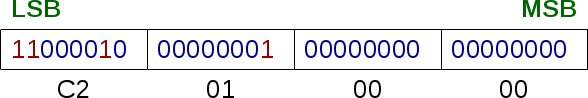
\includegraphics[width=0.9\textwidth]{imgs/little_endian.png}}
\end{frame}

\subsection{Investigando un juego}
\begin{frame}{Tinke}
    \only<1>{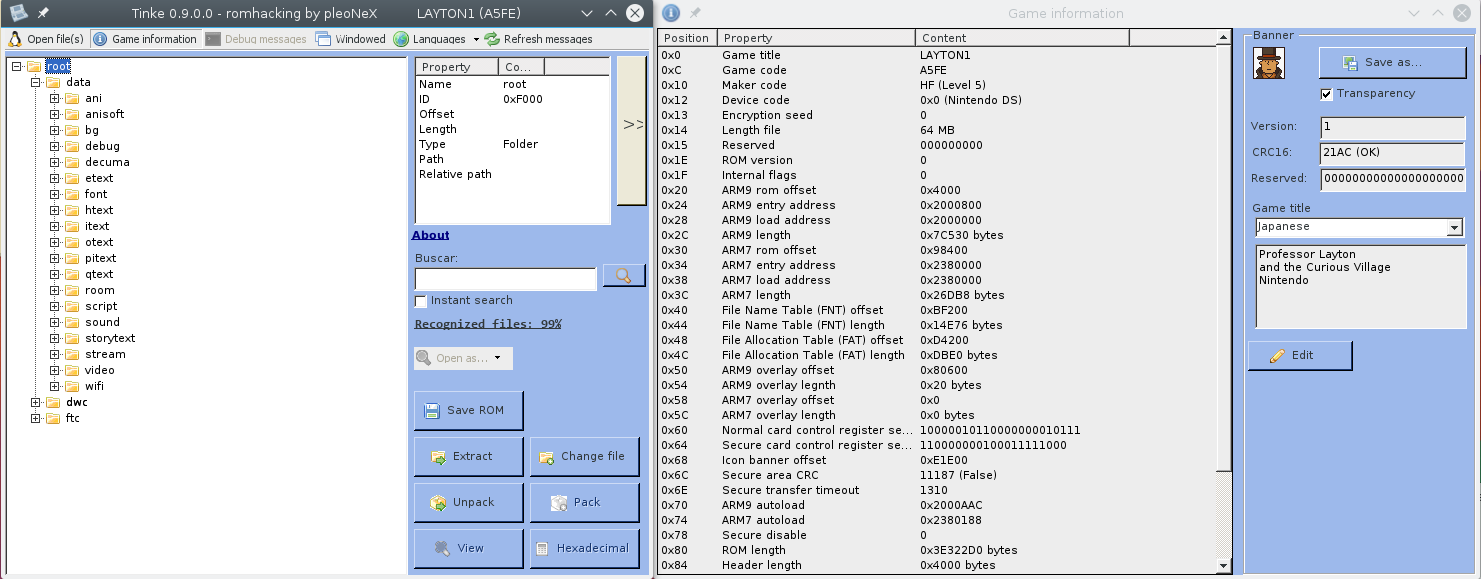
\includegraphics[width=\textwidth]{imgs/tinke.png}}
    \only<2>{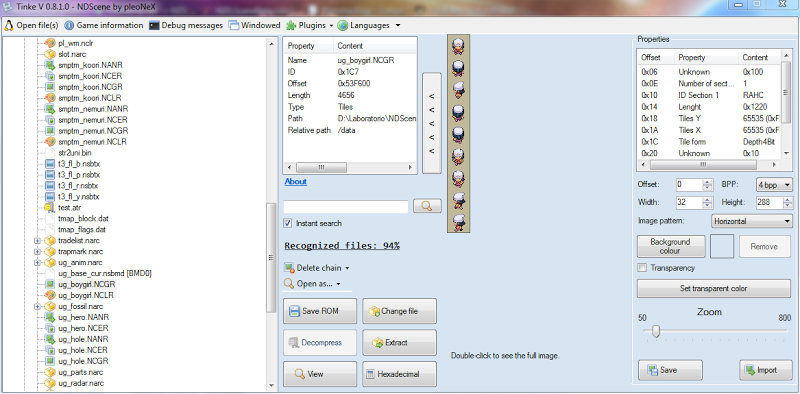
\includegraphics[width=\textwidth]{imgs/tinke_preview.png}}
\end{frame}

\begin{frame}{Tipos de ficheros}
    \begin{columns}
    \begin{column}{0.5\textwidth}
        \begin{itemize}
            \item 
\includegraphics{imgs/palette.png}~Paleta
            \item 
\includegraphics{imgs/picture.png}~Tiles
            \item 
\includegraphics{imgs/picture_link.png}~Map
            \item 
\includegraphics{imgs/pictures.png}~Sprites
            \item 
\includegraphics{imgs/picture_go.png}~Animaciones
            \item 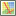
\includegraphics{imgs/map.png}~Modelos 3D
            \item 
\includegraphics{imgs/image.png}~Texturas
            \item 
\includegraphics{imgs/photo.png}~Imagen completa
        \end{itemize}
    \end{column}
    \hfill
    \begin{column}{0.5\textwidth}
        \begin{itemize}
            \item 
\includegraphics{imgs/page_white_text.png}~Texto
            \item 
\includegraphics{imgs/font.png}~Tipografía
            \item 
\includegraphics{imgs/script.png}~Scripts
            \item 
\includegraphics{imgs/compress.png}~Archivo comprimido
            \item 
\includegraphics{imgs/package.png}~Paquete
            \item 
\includegraphics{imgs/music.png}~Música
            \item 
\includegraphics{imgs/film.png}~Vídeo
        \end{itemize}
    \end{column}
    \end{columns}
\end{frame}

\subsection{Editar juegos}
\begin{frame}{Modificando textos}
    \begin{columns}
    \begin{column}{0.5\textwidth}
        \begin{enumerate}
            \item<1-> Localizar texto a modificar
            \item<2-> Abrir juego en Tinke
            \item<3-> Localizar textos
            \item<4-> Extraer archivo
            \item<5-> Modificar con editor
            \item<6-> Importar archivo
            \item<7-> Generar ROM
            \item<8-> Probar en DeSmuME
        \end{enumerate}
    \end{column}
    \hfill
    \begin{column}{0.5\textwidth}
        \centering
        \only<1>{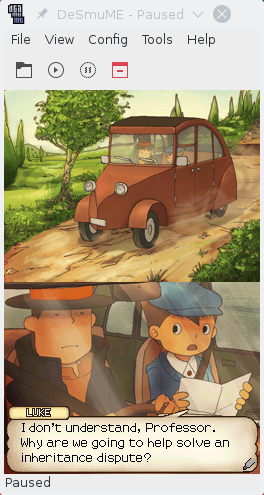
\includegraphics[width=0.7\textwidth]{imgs/mod1.png}}
        \only<2>{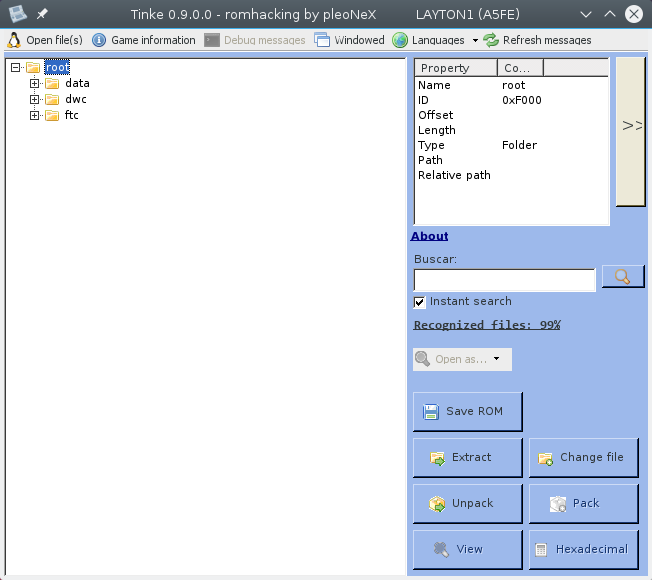
\includegraphics[width=\textwidth]{imgs/mod2.png}}
        \only<3>{\includegraphics[width=\textwidth]{imgs/mod3.png}}
        \only<4>{\includegraphics[width=\textwidth]{imgs/mod4.png}}
        \only<5>{\includegraphics[width=\textwidth]{imgs/mod5.png}}
        \only<6>{\includegraphics[width=\textwidth]{imgs/mod6.png}}
        \only<7>{\includegraphics[width=\textwidth]{imgs/mod7.png}}
        \only<8>{\includegraphics[width=0.7\textwidth]{imgs/mod8.png}}
        \only<9>{\includegraphics[width=0.7\textwidth]{imgs/pepino.png}}
    \end{column}
    \end{columns}
\end{frame}

\subsection{Publicar cambios}
\begin{frame}{Parches}
    \begin{columns}
    \begin{column}{0.6\textwidth}
        \small
        \begin{wideitemize}
            \item<1-> Solo contienen las modificaciones
            \item<2-> \textbf{No subir el juego modificado}
            \item<3-> Tamaño pequeño (entre 1 y 20 MB)
            \item<4-> Formatos comunes: IPS y xDelta
        \end{wideitemize}
    \end{column}
    \begin{column}{0.4\textwidth}
        \includegraphics[width=\textwidth]{imgs/ninopatcher.png}
    \end{column}
    \end{columns}
\end{frame}

\begin{frame}{xDelta}
    \begin{columns}
    \begin{column}{0.7\textwidth}
        \footnotesize
        \begin{wideitemize}
            \item<1-> Windows: xdelta UI \\ \url{http://www.romhacking.net/utilities/598/}

            \item<2-> Mac OS X: Multipatch \\ \url{http://projects.sappharad.com/tools/multipatch.html}

            \item<3-> Linux: xdelta
            \begin{itemize}
                \footnotesize
                \item Parchear: \\ \texttt{xdelta -d -s ORIGINAL PARCHE}
                \item Crear parche: \\ \texttt{xdelta -9 -s ORIGINAL MODIFICADO PARCHE}
            \end{itemize}
        \end{wideitemize}
    \end{column}
    \begin{column}{0.3\textwidth}
        \includegraphics[width=\textwidth]{imgs/xdelta_windows.png}
        \vfill
        \visible<2->{\includegraphics[width=\textwidth]{imgs/xdelta_mac.png}}
    \end{column}
    \end{columns}
\end{frame}

\section{Programas de edición}
\subsection{Pokémon}
\begin{frame}{Advanced Map}
    \centering
    \includegraphics[width=\textwidth]{imgs/advanced_map.png} \\
    Proyecto: \url{http://ampage.no-ip.info/}
\end{frame}

\begin{frame}{Spiky's DS Map Editor}
    \centering
    \includegraphics[width=0.85\textwidth]{imgs/sdme.png} \\
    Proyecto: \url{https://github.com/MarcRiera/SDSME}
\end{frame}

\subsection{New Super Mario Bros DS}
\begin{frame}{NSMB Editor}
    \centering
    \includegraphics[width=\textwidth]{imgs/nsmbe.png} \\
    Proyecto: \url{https://github.com/Dirbaio/NSMB-Editor}
\end{frame}

\subsection{Super Mario 64 DS}
\begin{frame}{Super Mario 64 Editor}
    \centering
    \includegraphics[width=0.9\textwidth]{imgs/sm64ds.png} \\
    Descarga: \url{http://www.romhacking.net/utilities/764}
\end{frame}

\subsection{Ni no kuni}
\begin{frame}{NinoCompiler}
    \begin{tikzpicture}
        \node<1-> (img1) at (0,0) {\includegraphics[width=\textwidth]{imgs/ninoscritor.png}};

        \node<2-> (img2) at (-1.2, 0.7) {\includegraphics[width=0.75\textwidth]{imgs/ninoxml.png}};
        \node<3-> (img3) at (2,-1) {\includegraphics[width=0.3\textwidth]{imgs/ninoimg.png}\huge\textrightarrow\includegraphics[width=0.3\textwidth]{imgs/ninoimg_trans.png}};
        \node<4-> (img4) at (0,0) {\includegraphics[width=0.5\textwidth]{imgs/ninocompiler.png}};
    \end{tikzpicture}

    \visible<4->{\centering
    Proyecto: \url{http://gradienwords.com} \\
    GitHub: \url{https://github.com/pleonex/Ninokuni}}
\end{frame}

    \section{Reto 1}
\begin{frame}{Reto 1}
    \Huge\centering\textbf{CHALLENGE TIME!}
\end{frame}

\subsection{Puzles en Profesor Layton}
\begin{frame}{Objetivo}

    {\Large\bfseries Modifica un puzle}
    \begin{columns}
    \begin{column}{0.5\textwidth}
        \begin{itemize}
            \item<1-> Descripción (\textit{qtext})
            \item<2-> Pistas (\textit{qtext})
            \item<3-> Solución (\textit{script/qscript})
            \item<4-> Confirmación (\textit{qtext})
        \end{itemize}
    \end{column}
    \begin{column}{0.5\textwidth}
        \only<1>{\includegraphics[width=0.7\textwidth]{imgs/reto1_1.png}}
        \only<2>{\includegraphics[width=0.7\textwidth]{imgs/reto1_2.png}}
        \only<3>{\includegraphics[width=0.7\textwidth]{imgs/reto1_3.png}}
        \only<4>{\includegraphics[width=0.7\textwidth]{imgs/reto1_4.png}}
    \end{column}
    \end{columns}

    \note[itemize]{
        \item Primeros 4 bytes es el tamaño del archivo
        \item Se compone de múltiples comandos + argumentos
        \item Después de \texttt{0x0000} va el ID del comando
        \item El formato de los argumentos es tipo + valor
        \item El tipo \texttt{0x0001} es un entero de 32 bits
        \item El tipo \texttt{0x0003} es una cadena de caracteres de longitud variable
        \item Los scripts terminan con \texttt{0x000C}
    }
\end{frame}

    \begin{frame}{Contenido}
    \begin{columns}
    \begin{column}{0.5\textwidth}
        \uncover<2->{\large Textos}
        \begin{itemize}
            \item<2-> Codificaciones
            \item<2-> Formatos
        \end{itemize}
        \uncover<2->{Tipografías}
        \visible<2->{\includegraphics[width=0.8\textwidth]{imgs/example_text.png}}
    \end{column}
    \hfill
    \begin{column}{0.5\textwidth}
        \uncover<3->{\large Imágenes}
        \begin{itemize}
            \item<3-> Fondos
            \item<3-> Sprites
            \item<3-> Texturas
        \end{itemize}
        \vfill{}
        \visible<3->{\includegraphics[width=0.8\textwidth]{imgs/example_img.png}}
    \end{column}
    \end{columns}
\end{frame}

\section{Textos}
\begin{frame}{Naturaleza de los textos}
    \centering\Large ¿Cómo guardamos texto de forma digital?
    \includegraphics[width=0.75\textwidth]{imgs/example_text.png}
\end{frame}

\subsection{Codificaciones}
\begin{frame}{Codificación de caracteres}
    \centering
    \only<1>{
        \begin{block}{}
            Es el método que permite convertir un carácter de un lenguaje natural en un símbolo de otro sistema de representación aplicando reglas de codificación. [Wikipedia]
        \end{block}
    }
    \only<2>{\includegraphics[width=\textwidth]{imgs/ascii-table.png}}
\end{frame}

\begin{frame}{ASCII}
    \begin{block}{}
        \centering Codifica caracteres del alfabeto latino en 7 bits.
    \end{block}
    \begin{columns}
    \begin{column}{0.40\textwidth}
        \includegraphics[trim={1616px 0 0 0},clip,width=\textwidth]{imgs/ascii-table.png}
    \end{column}
    \begin{column}{0.55\textwidth}
        \centering
        \includegraphics[width=\textwidth]{imgs/text_hex.png} \\
        \Huge \textdownarrow \\
        \includegraphics[width=0.7\textwidth]{imgs/text_hex1.png}
    \end{column}
    \end{columns}
\end{frame}

\begin{frame}{Latin-1 (ISO 8859-1)}
    \begin{block}{}
        Codificación extendida de ASCII. Utiliza 8 bits añadiendo 128 caracteres necesarios para las lenguas europeas.
    \end{block}
    \centering\includegraphics[width=0.75\textwidth]{imgs/latin1.png}
\end{frame}

\begin{frame}{Unicode}
    \begin{block}{}
        Estándar universal de codificación de caracteres para la mayoría de lenguas (incluidas las muertas). La última version 6.0 incluye 109.449 caracteres.
    \end{block}

    \begin{itemize}
        \item<2-> Unicode es solo una tabla, no especifica la codificación.
        \item<3-> Codificaciones para unicode:
        \begin{itemize}
            \item<4-> UTF-8: codificación de 8 bits de longitud variable.\\ \texttt{'A' = 41h, '}\visible<4->{\includegraphics[height=7px]{imgs/rare_char.png}}\texttt{' = F0 A0 9C 8E}
            \item<5-> UTF-16: codificación de 16 bits de longitud variable. \\ \texttt{'A' = 0041, '}\visible<5->{\includegraphics[height=7px]{imgs/rare_char.png}}\texttt{' = D841 DF0E}
            \item<6-> UTF-32: codificación de 8 bits de longitud fija. \\ \texttt{'A' = 00000041, '}\visible<6->{\includegraphics[height=7px]{imgs/rare_char.png}}\texttt{' = 0002070E}
        \end{itemize}
    \end{itemize}
\end{frame}

\begin{frame}{Shift Jis (CP 932)}
    \begin{block}{}
        Codificación de longitud variable (1 o 2 bytes) para caracteres japoneses. Incluye ASCII.
    \end{block}
    \includefigure{Tabla para caracteres con primer byte \texttt{0x82}}{imgs/shiftjis_table82.png}{0.55}
\end{frame}

\begin{frame}{Ejemplos en archivos}
    \centering\Large
    \only<1>{¿? \\}
    \only<2->{UTF-16 \\}
    \includegraphics[width=0.75\textwidth]{imgs/utf16.png} \\
    \only<3>{¿? \\}
    \only<4->{Shift Jis \\}
    \visible<3->{\includegraphics[width=0.75\textwidth]{imgs/shiftjis.png}}
\end{frame}

\begin{frame}{Tablas}
    Algunos juegos usan codificaciones propietarias...
    \begin{itemize}
        \item ... fácil \textit{mapeo} con la tipografía.
        \item ... dificultar el acceso.
    \end{itemize}
    \includefigure{Textos de Pokémon Perla}{imgs/text_perla.png}{1}
\end{frame}

\begin{frame}[t,fragile]{Tablas}
    \includegraphics[width=\textwidth]{imgs/text_perla_trans.png}
    \footnotesize\ctable[]{cc|cc|cc}{}{                                     \FL
Valor          & Caracter & Valor          & Caracter & Valor    & Caracter \ML
\texttt{01A9h} & ¡        & \texttt{01ABh} & !        & \texttt{01ADh} & ,  \NN
\texttt{01DEh} & \textit{SP} & \texttt{E000h} & \textit{NL} & \texttt{0152h} & E \NN
\texttt{0132h} & H        & \texttt{013Ah} & P        & \texttt{013Eh} & T  \NN
\texttt{0145h} & a        & \texttt{0147h} & c        & \texttt{0148h} & d  \NN
\texttt{014Ch} & h        & \texttt{0150h} & l        & \texttt{0152h} & n  \NN
\texttt{0153h} & o        & \texttt{0156h} & r        & \texttt{0158h} & t  \LL
    }
\end{frame}

\subsection{Formatos}
\begin{frame}{Punteros (\textit{offsets})}
    \begin{block}{}
        \centering{}Número enteros que indican la posición del texto.
    \end{block}
    \vfill{}
    \uncover<2->{\large Tipos:}
    \begin{itemize}
        \item<3-> \textit{Absoluto}: desde el comienzo del archivo.
        \item<4-> Relativo: desde otra posición
        \begin{itemize}
            \item Relativo a una sección del fichero.
            \item Relativo a la posición actual.
        \end{itemize}
    \end{itemize}
\end{frame}

\begin{frame}{Punteros (\textit{offsets})}
    \centering\Large Formato \texttt{BMG}
    \vfill{}
    \begin{tikzpicture}
        \node[anchor=south west,inner sep=0] (image) at (0,0)
        {\includegraphics[width=\textwidth]{imgs/pointers.png}};
            \begin{scope}[x={(image.south east)},y={(image.north west)}]
                \draw[black,thick] (0.775,0) -- (0.775,1);
                \draw<2-4>[red,semithick] (0.13,0.9) rectangle (1,0.57);
                \draw<2-4>[blue,semithick] (0.13,0.565) rectangle (1,0.0);
                \draw<3,4>[blue,semithick] (0.13,0.565) rectangle (0.446,0.495);
                \draw<4->[blue,line width=2pt,->] (0.446,0.65) -- (0.446,0.55);
                \draw<5,6>[red,semithick] (0.13,0.81) rectangle (0.29,0.745);
                \draw<6>[blue,semithick] (0.765,0.565) -- (0.53,0.565) -- (0.53,0.495) -- (0.765,0.495);
                \draw<6>[blue,semithick] (1,0.565) -- (0.913,0.565) -- (0.913,0.495) -- (1,0.495);
                \draw<6>[blue,semithick] (0.78,0.49) -- (0.835,0.49) -- (0.835,0.41) -- (0.78,0.41);
                \draw<6>[blue,semithick] (0.13,0.49) -- (0.29,0.49) -- (0.29,0.41) -- (0.13,0.41);
                \draw<7,8>[red,semithick] (0.45,0.81) rectangle (0.60,0.745);
                \draw<8,9>[blue,semithick] (0.13, 0) -- (0.13, 0.4) -- (0.29, 0.4) -- (0.29,0.49) -- (0.765, 0.49) -- (0.765, 0);
                \draw<8,9>[blue,semithick] (0.78, 0) -- (0.78, 0.4) -- (0.835, 0.4) -- (0.835, 0.49) -- (1, 0.49) -- (1, 0);
                \draw<9>[green,semithick] (0.21, 0.49) rectangle (0.29, 0.4);
                \draw<9>[green,semithick] (0.37, 0.4) rectangle (0.445, 0.32);
                \draw<9>[green,semithick] (0.37, 0.24) rectangle (0.445, 0.16);
            \end{scope}
    \end{tikzpicture}
\end{frame}

\section{Imágenes}
\begin{frame}{Naturaleza de las imágenes}
    \centering\Large ¿Qué necesitamos para formar una imagen?
    \includegraphics[width=0.75\textwidth]{imgs/example_img.png}
\end{frame}

\subsection{Imágenes de fondo}
\begin{frame}{Partes de una imagen}
    \begin{block}{}
        \centering{}Una imagen se compone de sucesión de colores (píxeles).
    \end{block}
    \vfill{}
    \begin{columns}
    \begin{column}{0.25\textwidth}
        \visible<2->{\includegraphics[width=\textwidth]{imgs/zelda_pal.png}}
    \end{column}
    \begin{column}{0.05\textwidth}
        \visible<3->{\huge +}
    \end{column}
    \begin{column}{0.5\textwidth}
        \visible<3->{\includegraphics[width=\textwidth]{imgs/zelda_px.png}}
    \end{column}
    \begin{column}{0.05\textwidth}
        \visible<4->{\huge =}
    \end{column}
    \begin{column}{0.25\textwidth}
        \visible<4->{\includegraphics[width=\textwidth]{imgs/example_img.png}}
    \end{column}
    \end{columns}
\end{frame}

\begin{frame}{Colores}
    \begin{block}{}
        Los colores se forman \textit{mezclando} los tres colores base (componentes / canal): \textbf{rojo}, \textbf{verde} y \textbf{azul}.
    \end{block}
    \begin{columns}
    \begin{column}{0.2\textwidth}
        \centering
        \includegraphics[width=\textwidth]{imgs/rgb.png}
    \end{column}
    \begin{column}{0.8\textwidth}
        \small
        \begin{itemize}
            \item<2-> El rango de valores de cada componente define los colores únicos.
            \item<3-> Generalmente: 8 bits/canal \\
            $2^8=256\rightarrow 256^3=16.777.216$ colores únicos.
            \item<4-> NDS: 5 bits (\texttt{BGR555}) $\rightarrow$ 32.768 colores únicos.
            \begin{itemize}
                \item<4-> Un color ocupa 16 bits:\\
                5 por canal + 1 transparencia.
            \end{itemize}
        \end{itemize}
    \end{column}
    \end{columns}
\end{frame}

\begin{frame}{Paletas}
    \begin{block}{}
        Agrupación de colores. Definen los colores de una imagen. El primer color suele ser el transparente.
    \end{block}
    {\centering\includegraphics[width=0.25\textwidth]{imgs/zelda_pal.png}\\}
    \uncover<2->{Modalidades:}
    \begin{itemize}
        \item<2-> 1 paleta de 256 colores = 256 colores.
        \item<3-> 16 paletas de 16 colores = 256 colores.
        \item<4-> 16 paletas de 256 colores = 4.096 colores.
    \end{itemize}
\end{frame}

\begin{frame}{Píxeles}
    \begin{block}{}
        La información que guardamos por píxel es la posición en la paleta de su color.
    \end{block}
    {\centering\includegraphics[width=0.25\textwidth]{imgs/zelda_px.png}\\}
    \uncover<2->{Codificaciones:}
    \begin{itemize}
        \item<2-> 8 bits por píxel (bpp): $2^8=256$ posiciones diferentes $\rightarrow$ 256 colores diferentes.
        \item<3-> 4 bpp: 16 colores diferentes.
        \item<4-> 1 bpp: 2 colores diferentes (blanco o negro).
    \end{itemize}
\end{frame}

\begin{frame}{Agrupación de píxeles}
    \centering
    \only<1,3>{
    \begin{tikzpicture}
        \node[anchor=south west,inner sep=0] (image) at (0,0)
        {\includegraphics[width=256px]{imgs/example_img.png}};
        \begin{scope}[x={(image.south east)},y={(image.north west)}]
            \draw<3>[help lines,xstep=8bp,ystep=8bp] (0,0) grid (1,1);
        \end{scope}
    \end{tikzpicture}
    }
    \only<2>{
    \includegraphics[width=\textwidth]{imgs/img_lineal.png}
    }
\end{frame}

\begin{frame}[fragile]{Agrupación de píxeles}
    \begin{columns}
    \begin{column}{0.1\textwidth}
        \begin{tikzpicture}
            \node[anchor=south west,inner sep=0] (image) at (0,0)
            {\includegraphics[width=16px]{imgs/small_img.png}};
            \begin{scope}[x={(image.south east)},y={(image.north west)}]
                \draw[help lines,xstep=8bp,ystep=8bp] (0,0) grid (1,1);
            \end{scope}
        \end{tikzpicture}
    \end{column}
    \begin{column}{0.9\textwidth}
        {\textbf{Lineal}}
        \begin{lstlisting}[basicstyle=\ttfamily\footnotesize]
00 01 02 03 04 05 06 07 08 09 0A 0B 0C 0D 0E 0F
10 11 12 13 14 15 16 17 18 19 1A 1B 1C 1D 1E 1F
20 21 22 23 24 25 26 27 28 29 2A 2B 2C 2D 2E 2F
30 31 32 33 34 35 36 37 38 39 3A 3B 3C 3D 3E 3F
40 41 42 43 44 45 46 47 48 49 4A 4B 4C 4D 4E 4F
        \end{lstlisting}
        \begin{uncoverenv}<2->{\textbf{Horizontal}}
        \begin{lstlisting}[basicstyle=\ttfamily\footnotesize\color{red},
            belowskip=-0.5\baselineskip]
00 01 02 03 04 05 06 07 10 11 12 13 14 15 16 17
20 21 22 23 24 25 26 27 30 31 32 33 34 35 36 37
40 41 42 43 44 45 46 47 50 51 52 53 54 55 56 57
60 61 62 63 64 65 66 67 70 71 72 73 74 75 76 77\end{lstlisting}
        \begin{lstlisting}[basicstyle=\ttfamily\footnotesize\color{blue}]
08 09 0A 0B 0C 0D 0E 0F 18 19 1A 1B 1C 1D 1E 1F
        \end{lstlisting}\end{uncoverenv}
    \end{column}
    \end{columns}
\end{frame}

\begin{frame}{Compresión}
    \only<1>{
    \centering
    \begin{tikzpicture}
        \node[anchor=south west,inner sep=0] (image) at (0,0)
        {\includegraphics[width=256px]{imgs/zelda_nintendo.png}};
        \begin{scope}[x={(image.south east)},y={(image.north west)}]
            \draw[help lines,xstep=8bp,ystep=8bp] (0,0) grid (1,1);
        \end{scope}
    \end{tikzpicture}
    }
    \only<2-4>{
    \centering
    \begin{columns}
    \begin{column}{0.15\textwidth}
        \begin{tikzpicture}
            \node[anchor=south west,inner sep=0] (image) at (0,0)
            {\includegraphics[width=48px]{imgs/zelda_nintendo_compress.png}};
            \begin{scope}[x={(image.south east)},y={(image.north west)}]
                \draw[help lines,xstep=8bp,ystep=8bp] (0,0) grid (1,1);
            \end{scope}
        \end{tikzpicture}
    \end{column}
    \begin{column}{0.05\textwidth}
        \visible<3->{\huge +}
    \end{column}
    \begin{column}{0.5\textwidth}
        \visible<3->{\includegraphics[width=\textwidth]{imgs/screen_info.png}}
    \end{column}
    \begin{column}{0.05\textwidth}
        \visible<4->{\huge =}
    \end{column}
    \begin{column}{0.25\textwidth}
        \visible<4->{\includegraphics[width=\textwidth]{imgs/zelda_nintendo.png}}
    \end{column}
    \end{columns}
    }
    \only<5-6>{
    \begin{columns}
    \begin{column}{0.5\textwidth}
        \centering
        \includegraphics[width=0.7\textwidth]{imgs/map_ninokuni_mess.png}
    \end{column}
    \begin{column}{0.05\textwidth}
        \visible<6->{\huge$\rightarrow$}
    \end{column}
    \begin{column}{0.5\textwidth}
        \centering
        \visible<6->{
        \includegraphics[width=0.7\textwidth]{imgs/map_ninokuni_fix1.png} \\
        \vspace{10pt}
        \includegraphics[width=0.7\textwidth]{imgs/map_ninokuni_fix2.png}
        }
    \end{column}
    \end{columns}
    }
    \only<7->{
    Compresión de \textit{tiles}:
    \begin{itemize}
        \item<7-> Evita guardar \textit{tiles} idénticos.
        \item<8-> Evita guardar \textit{tiles volteados} horizontalmente o verticalmente.
        \item<9-> Permite agrupar imágenes.
        \item<10-> Permite usar 256 colores distintos en formatos 4bpp.
        \begin{itemize}
            \item<11-> Cada \textit{tile} usa una paleta.
        \end{itemize}
    \end{itemize}
    }
\end{frame}

\subsection{Sprites}
\begin{frame}{Casos de uso}
    \only<1-4>{
    \begin{columns}
    \begin{column}{0.5\textwidth}
        \centering
        \textbf{Capas} \\ \vspace{10pt}
        \only<1>{\includegraphics[width=\textwidth]{imgs/zelda_title.png}}
        \only<2->{\includegraphics[width=\textwidth]{imgs/zelda_title_cells.png}}
    \end{column}
    \hfill
    \begin{column}{0.5\textwidth}
        \centering
        \uncover<3->{\textbf{Animaciones}} \\ \vspace{10pt}
        \visible<3->{\includegraphics[width=30px]{imgs/zelda_anm-0.png}}
        \visible<4>{
        \vfill{}
        \includegraphics[width=30px]{imgs/zelda_anm-1.png}\hfill{}
        \includegraphics[width=30px]{imgs/zelda_anm-2.png}\hfill{}
        \includegraphics[width=30px]{imgs/zelda_anm-3.png}
        }
    \end{column}
    \end{columns}
    }

    \only<5>{
    \centering
    \textbf{Ahorro de espacio con capas}
    \vfill{}
    \begin{columns}
    \begin{column}{0.25\textwidth}
        \includegraphics[width=\textwidth]{imgs/zelda_btn_base.png}
    \end{column}
    \begin{column}{0.05\textwidth}
        \huge +
    \end{column}
    \begin{column}{0.2\textwidth}
        \includegraphics[width=\textwidth]{imgs/zelda_btn_text1.png}
        \vspace{10pt}
        \includegraphics[width=\textwidth]{imgs/zelda_btn_text2.png}
    \end{column}
    \begin{column}{0.05\textwidth}
        \huge =
    \end{column}
    \begin{column}{0.25\textwidth}
        \includegraphics[width=\textwidth]{imgs/zelda_btn1.png}
        \vspace{10pt}
        \includegraphics[width=\textwidth]{imgs/zelda_btn2.png}
    \end{column}
    \end{columns}
    }
\end{frame}

\begin{frame}{Formatos base}
    \begin{columns}
    \begin{column}{0.45\textwidth}
        \centering{}Paleta \\ \vspace{5pt}
        \includegraphics[width=\textwidth]{imgs/zelda_title_pal.png}
    \end{column}
    \begin{column}{0.05\textwidth}
        \uncover<2>{\huge +}
    \end{column}
    \begin{column}{0.45\textwidth}
        \centering{}\uncover<2>{\textit{Tiles}} \\ \vspace{5pt}
        \visible<2>{\includegraphics[width=\textwidth]{imgs/zelda_title_px.png}}
    \end{column}
    \end{columns}
\end{frame}

\begin{frame}{Celdas}
    \centering{}Nitro CElls Resource (.ncer) \\ \vspace{5pt}
    \includegraphics[width=0.6\textwidth]{imgs/zelda_title_ui.png}
\end{frame}

\begin{frame}{Animaciones}
    \centering{}Nitro AnimatioN Resource (.nanr) \\ \vspace{5pt}
    \includegraphics[width=0.6\textwidth]{imgs/zelda_anm_ui.png}
\end{frame}

\subsection{3D}
\begin{frame}{Texturas}
    \centering{}Nitro TeXture (.nsbtx) \\ \vspace{5pt}
    \begin{columns}
    \begin{column}{0.5\textwidth}
        \only<1-3>{\includegraphics[width=\textwidth]{imgs/zelda_link_tex.png}}
        \only<4>{\includegraphics[width=\textwidth]{imgs/zelda_house_tex.png}}
    \end{column}
    \begin{column}{0.6\textwidth}
        \begin{wideitemize}
            \item<1-> Uso en modelos 3D
            \item<2-> Paletas + \textit{Tiles}
            \item<3-> Codificaciones: A3I5, A4I4, A5I3, 4x4 texel
        \end{wideitemize}
    \end{column}
    \end{columns}
\end{frame}

\begin{frame}{Modelos 3D}
    \begin{columns}
    \begin{column}{0.5\textwidth}
        \begin{wideitemize}
            \item<1-> Geometría 3D.
            \item<2-> Comandos de OpenGL 1.0.
        \end{wideitemize}
    \end{column}
    \begin{column}{0.6\textwidth}
        \only<1-2>{\includegraphics[width=\textwidth]{imgs/zelda_house.png}}
        \only<3>{\includegraphics[width=\textwidth]{imgs/zelda_map.png}}
    \end{column}
    \end{columns}
\end{frame}

\section{Tipografías y audios}
\subsection{Tipografías y audios}
\begin{frame}{Tipografías}
    \centering{}Nitro FonT Resource (.nftr) \\ \vspace{5pt}
    \begin{columns}
    \begin{column}{0.5\textwidth}
        \includegraphics[width=\textwidth]{imgs/zelda_font.png}
    \end{column}
    \begin{column}{0.6\textwidth}
        \begin{wideitemize}
            \item<+-> Una imagen por caracter.
            \item<+-> Mapeo binario $\leftrightarrow$ imagen.
            \item<+-> Tabla + Imágenes.
            \item<+-> Útil para reemplazo de caracteres.
        \end{wideitemize}
    \end{column}
    \end{columns}
\end{frame}

\begin{frame}{Audios}
    \centering{}Sound DATa (.sdat) \\ \vspace{5pt}
    \begin{columns}
    \begin{column}{0.6\textwidth}
        \begin{wideitemize}
            \item<+-> Sonido digitalizado (STRM).
            \begin{itemize}
                \item<+-> PCM, ADPCM, Procyon.
                \item<+-> Mono y estéreo.
                \item<+-> Sample format: 4 a 16 bits.
                \item<+-> Sample rate: 16 KHz, 32 KHz.
                \item<+-> Bucles.
            \end{itemize}
            \item<+-> Sonido sintetizado (SSEQ).
            \begin{itemize}
                \item<+-> Partitura: SSEQ.
                \item<+-> Notas musicales: SBNK, SWAR.
            \end{itemize}
        \end{wideitemize}
    \end{column}
    \begin{column}{0.5\textwidth}
        \includegraphics[width=\textwidth]{imgs/zelda_music.png}
    \end{column}
    \end{columns}
\end{frame}

    \section{Reto 2}
\begin{frame}{Reto 2}
    \Huge\centering\textbf{CHALLENGE TIME!}
\end{frame}

\subsection{The Legend of Zelda: Phantom Hourglass}
\begin{frame}[t]{Contenido sorpresa}
    \begin{columns}
    \begin{column}[T]{0.5\textwidth}
        \centering
        \visible<2->{¿\textit{/Test/picture.narc}?\\\vspace{5pt}}
        \visible<3->{\includegraphics[width=\textwidth]{imgs/zelda_dog.png}}
    \end{column}
    \hfill
    \begin{column}[T]{0.5\textwidth}
        \centering
        \visible<4->{¿\textit{/Test/BgMap.narc}?\\\vspace{5pt}}
        \visible<5->{\includegraphics[width=0.5\textwidth]{imgs/zelda_batch.png}}
    \end{column}
    \end{columns}
\end{frame}

\begin{frame}{Historia}
    \begin{columns}
    \begin{column}{0.5\textwidth}
        \begin{itemize}
            \item<1-> Modificar cuarto diálogo.
            \item<2-> Modificar imagen.
        \end{itemize}
        \vfill{}
        \hfill{}
        \visible<3->{\includegraphics[width=0.4\textwidth]{imgs/reto2_3.png}}
    \end{column}
    \begin{column}{0.5\textwidth}
        \visible<1->{\includegraphics[width=0.4\textwidth]{imgs/reto2_1.png}}
        \hfill{}
        \visible<2->{\includegraphics[width=0.4\textwidth]{imgs/reto2_2.png}}
        \vfill{}
        \begin{itemize}
            \item<3-> Modificar tipografía.
        \end{itemize}
    \end{column}
    \end{columns}
\end{frame}

\begin{frame}{Historia: Punteros}
    \begin{columns}
    \begin{column}{0.3\textwidth}
        \includegraphics[width=\textwidth]{imgs/reto2_1.png}
    \end{column}
    \begin{column}{0.7\textwidth}
        Modificar cuarto diálogo.
        \footnotesize
        \begin{itemize}
            \item Ruta: \textit{/Spanish/Message/demo.bmg}.
            \item Punteros en la sección \texttt{INF1} (cabecera: 16 B).
            \item Hay \texttt{0x08} bytes por texto.
            \item Primeros \texttt{0x04} bytes es el puntero.
            \item Puntero \textit{i}: $Offset_{INF1} + 16 + i*8=48h$.
            \item Punteros relativos a \texttt{0x0AE8}.
            \item Ignorar 6 bytes después de \texttt{001Ah}.
            \item Añadir pausa al final con: \\
                  \texttt{1A 00 08 01 0E 00 7D 00}.
        \end{itemize}
    \end{column}
    \end{columns}
\end{frame}

\begin{frame}{Historia: Imágenes}
    \begin{columns}
    \begin{column}{0.7\textwidth}
        Modificar imagen
        \footnotesize
        \begin{wideitemize}
            \item Ruta: \textit{/Event/Kamishibai/kami1/kami1-01}.
            \item Seleccionar \textit{Replace palette}.
            \item Importar imagen con mismas dimensiones:
            \begin{itemize}
                \item Ancho: \texttt{256} píxeles.
                \item Alto: \texttt{192} píxeles.
            \end{itemize}
        \end{wideitemize}
    \end{column}
    \begin{column}{0.3\textwidth}
        \includegraphics[width=\textwidth]{imgs/reto2_2.png}
    \end{column}
    \end{columns}
\end{frame}

\begin{frame}{Historia: Tipografía}
    \begin{columns}
    \begin{column}{0.3\textwidth}
        \includegraphics[width=\textwidth]{imgs/reto2_3.png}
    \end{column}
    \begin{column}{0.7\textwidth}
        Modificar tipografía
        \footnotesize
        \begin{wideitemize}
            \item Cambiar primer texto por:\\
                  $\int2x dx=x^2+K$
            \item Tipografía: \textit{/Font/zeldaDS\_15.nftr}.
            \item Reemplazar caracteres japoneses por: $\int$ y $^2$
        \end{wideitemize}
    \end{column}
    \end{columns}
\end{frame}


\end{document}
